\documentclass{article}

\usepackage{polski}
\usepackage[utf8]{inputenc}
\usepackage{booktabs}
\usepackage{biblatex}
\usepackage{subfigure}
\usepackage{graphicx}
\usepackage{float}
\usepackage{geometry}
\usepackage{listings}

 \usepackage[table,xcdraw]{xcolor}

\geometry{
	a4paper,
	total={170mm,257mm},
	left=50mm,
	right=50mm,
	top=45mm,
	bottom = 45mm
}
\usepackage{tabularx}


\lstset{
    language=R,   
    extendedchars=true,
    inputencoding=latin1,
     basicstyle=\small
}



\begin{document}
	\newgeometry{tmargin=4cm, bmargin=4cm, lmargin=3cm, rmargin=3cm}
	
	\begin{titlepage}
		\center
		\newcommand{\HRule}{\rule{\linewidth}{0.6mm}}
		
		\textsc{\LARGE Politechnika Wrocławska}\\[1.5cm]
		\textsc{\Large Laboratorium}\\[0.5cm] 
		\textsc{\large Inteligencja Obliczeniowa i jej Zastosowania}\\[0.7cm] 

		\HRule \\[0.4cm]
		{ \huge \bfseries Algorytmy ewolucyjne i hybrydowe}\\[0.4cm]
		\HRule \\[1.5cm]
		
		\begin{minipage}{0.4\textwidth}
			\begin{flushleft} \large
				\emph{Authors:}\\
				Rafał \textsc{Pieniążek}\\
                Jakub \textsc{Pomykała}
			\end{flushleft}
		\end{minipage}
		~
		\begin{minipage}{0.4\textwidth}
			\begin{flushright} \large
				\emph{Supervisor:} \\
				dr hab. inż. Olgierd \textsc{Unold}, prof. PWr
			\end{flushright}
		\end{minipage}\\[4cm]

		{\large \today}\\[3cm]
		
		\vfill
		
	\end{titlepage}
\tableofcontents
\newpage
\listoffigures
\newpage
\section{Wstęp}
	Celem laboratorium było przeprowadzenie optymalizacji globalnej dla wybranych funkcji z pakietu globalOptTests.
    

\section{Zastosowany algorytm optymalizacji}

W laboratorium zastosowano algorytmy genetyczne będące klasą algorytmów ewolucyjnych.
Algorytmy ewolucyjne stanowią kierunek sztucznej inteligencji, która wykorzystuje i symuluje ewolucję biologiczną. Wszystkie algorytmy tej klasy symulują podstawowe zachowania w teorii ewolucji biologicznej - procesy selekcji, mutacji i reprodukcji. Zachowanie jednostek zależy od środowiska. Zbiór jednostek nazywa się populacją. Taka populacja ewoluuje zgodnie z regułami selekcji zgodnie z funkcją celu przypisaną do środowiska. Propagowane do kolejnych pokoleń są tylko najbardziej dopasowane osobniki.


\subsection{Zastosowane narzędzia implementacji}

\subsubsection{Język R}
R jest językiem programowania i środowiskiem programistycznym, używanym głównie do obliczeń statystycznych i wizualizacji danych, do sztucznej inteligencji a także do ekonomii i innych zagadnień wykorzystujących obliczenia numeryczne. Został stworzony przez Rossa Ihakę i Roberta Gentlemana na Uniwersytecie w Auckland w Nowej Zelandii. 


\subsubsection{Pakiet GA}

Pakiet GA zawiera zestaw funkcji ogólnego przeznaczenia do optymalizacji z wykorzystaniem algorytmów genetycznych. Dostępnych jest kilka operatorów genetycznych, których można łączyć w celu zbadania najlepszych ustawień dla bieżącego zadania.


\subsubsection{Pakiet globalOpts}
Pakiet zawierający implementację funkcji przydatnych do przeprowadzania testów wydajnościowych algorytmów optymalizacji globalnej.

\newpage
\section{Własne operatory krzyżowania i mutacji}
\subsection{Funkcja wielomodalna - Funkcja Shuberta}
	\subsubsection{Wzór analityczny}
	   \begin{figure}[!htbp]
    \centering
    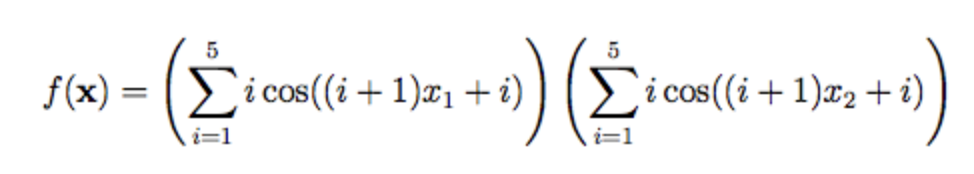
\includegraphics[width=0.6\textwidth]{inc/wzory/schubert}
     \caption{Wzór analityczny funkcji Schuberta}
    \end{figure}
    
    

    \subsubsection{Wykres w ustalonym przedziale zmiennych}
    
    \begin{figure}[!htbp]
    \centering
    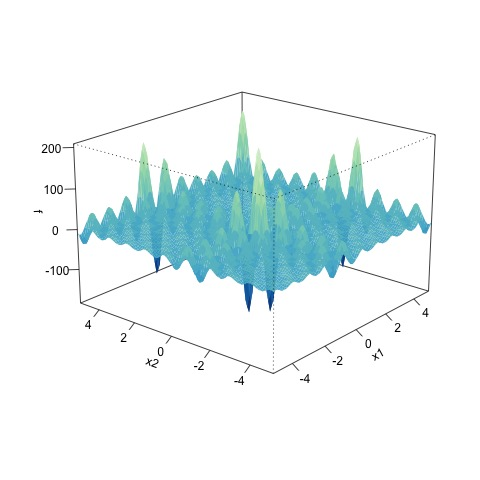
\includegraphics[width=0.6\textwidth]{inc/wykresyfunkcji/schubert}
     \caption{Wykres  funkcji Schuberta}
    \end{figure}
    
   

    \subsubsection{Ekstremum globalne}
    
       \begin{figure}[!htbp]
    \centering
    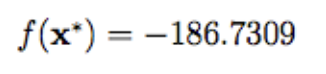
\includegraphics[width=0.3\textwidth]{inc/wzory/schubert-global-minimum}
     \caption{Minimum globalne dla funkcji Schuberta}
    \end{figure}
    
       \begin{figure}[!htbp]
    \centering
    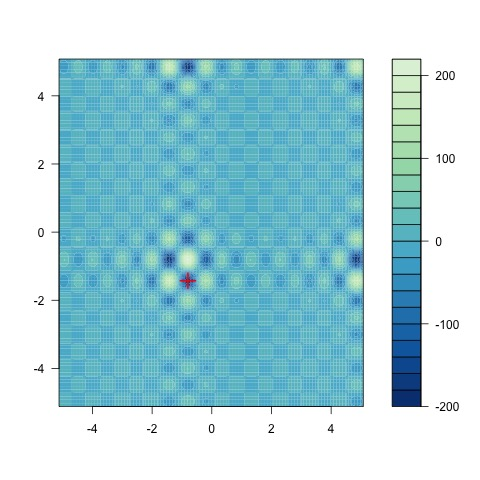
\includegraphics[width=0.7\textwidth]{inc/wykresyfunkcji/schubert-global-minimum}
     \caption{Minimum globalne dla funkcji Schuberta}
    \end{figure}
    

    

\subsection{Zmiana funkcji mutowania}
Poniżej przedstawiono własną propozycję implementacji funkcji mutowania.

\begin{lstlisting}
customMutation <- function(object, parent)
    {
      mod <- parent %% 2
      if(mod == 0){
        return (parent * 2)
      } else {
        return (parent / 2) + 1
      }
    }
\end{lstlisting}

	Na poniższych wykresach przedstawiono zestawienie rezultatów działania w przypadku domyślnej i własnej, zaimplementowanej funkcji mutacji. Wyniki dla funkcji domyślnej znajdują się po lewej stronie.
	
 	\begin{figure}[!h]
    \centering
    \mbox{
    \subfigure{
    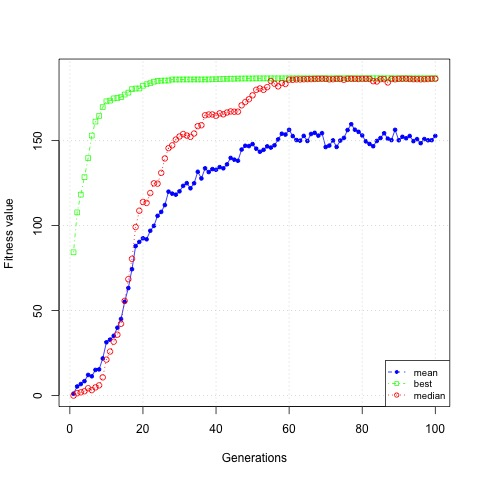
\includegraphics[width=3in]{{{inc/results/default_ga}}}\quad
    }
    \subfigure{
    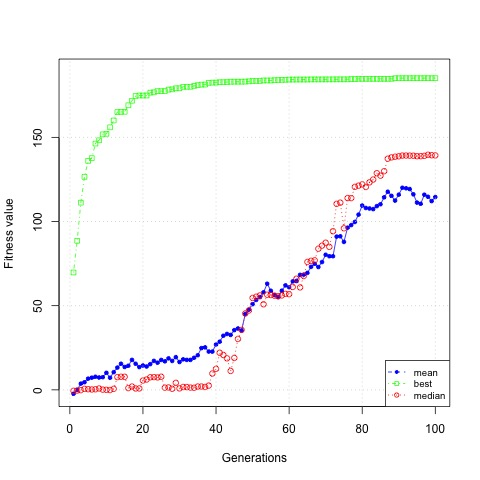
\includegraphics[width=3in]{{{inc/results/custom-mutation}}}\quad
    }
    }
    \caption{Porównanie domyślnej funkcji mutowania z własną}
    \end{figure}
    
     \begin{figure}[!h]
    \centering
    \mbox{
    \subfigure{
    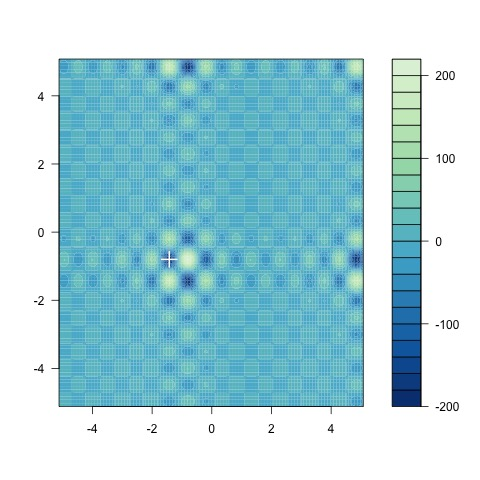
\includegraphics[width=3in]{{{inc/results/default_ga_result}}}\quad
    }
    \subfigure{
    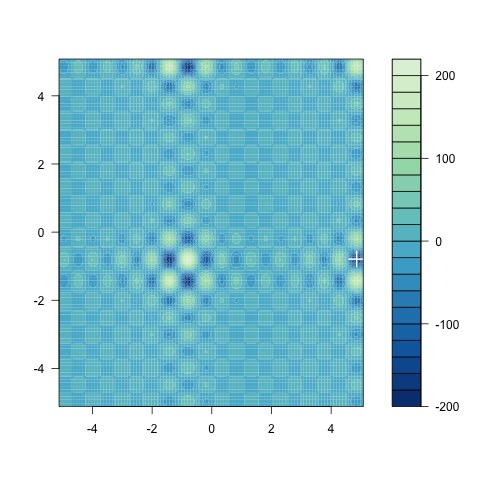
\includegraphics[width=3in]{{{inc/results/custom-mutation-result}}}\quad
    }
    }
    \caption{Porównanie domyślnej funkcji mutowania z własną - znalezione ekstrema}
    \end{figure}
    
    \newpage 
   Zmiana funkcji mutującej nie wpłynęła znacząco na wyniki końcowy. Mimo, iż w początkowej fazie wynik funkcji zbiegał do ekstremum wolniej niż w przypadku funkcji domyślnej, po 100 pokoleniach wynik jest na podobnym poziomie w obu przypadkach. Finalnie jednak algorytm z własną funkcją mutującą nie znalazł ekstremum globalnego. Widoczne jest to na wykresie temperaturowym, na którym zaznaczono rozwiązanie znalezione przez algorytm.
   
 W przypadku funkcji z własną funkcją mutowania można zauważyć spadek średniej i mediany wyników. Jest to spowodowane tym że dane zostają wyznaczane stochastycznie przez pakiet GA, a ich modyfikacja przez pomnożenie lub podzielenie przez stałą liczbę nie może poprawić ani pogorszyć wyniku w tym przypadku. Jakość znalezionych rozwiązań będzie mocno skorelowana z pierwotnie wyznaczonymi wartościami.
  

\subsection{Zmiana funkcji krzyżowania}
Poniżej przedstawiono własną propozycję implementacji funkcji krzyżowania.

\begin{lstlisting}
customCrossover <- function(object, parents)
    {
      parent_1 <- parents[[1]]
      parent_2 <- parents[[2]] 
      wektor_1 <- c(parent_1, parent_2)
      fitness = testFunctionWrapper(parent_1, parent_2)
      
      tmp_parent_1 <- parents[[1]] + runif(1, -1, 1)
      tmp_parent_2 <- parents[[2]] + runif(1, 1, -1)
      tmp_wektor_1 <- c(parent_1, parent_2)
      tmp_fitness = testFunctionWrapper(parent_1, parent_2)
      
      if(tmp_fitness > fitness){
        return (list(children=matrix(tmp_wektor_1), fitness=tmp_fitness))
      }
      return (list(children=matrix(wektor_1), fitness=fitness))
    }
\end{lstlisting}

	Na poniższych wykresach przedstawiono porównanie rezultatu działania algorytmu w przypadku zmiany funkcji krzyżowania z domyślnej na własną implementację. 
	
    \begin{figure}[!h]
    \centering
    \mbox{
    \subfigure{
    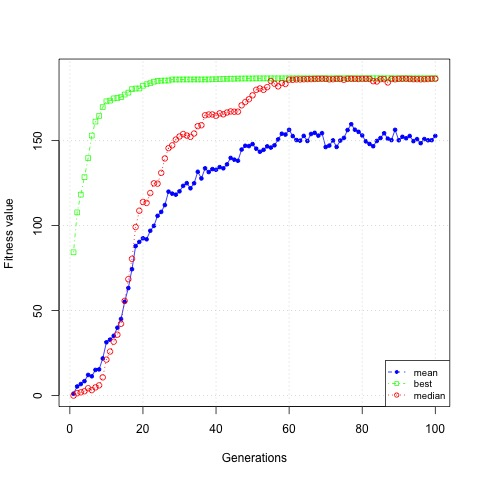
\includegraphics[width=3in]{{{inc/results/default_ga}}}\quad
    }
    \subfigure{
    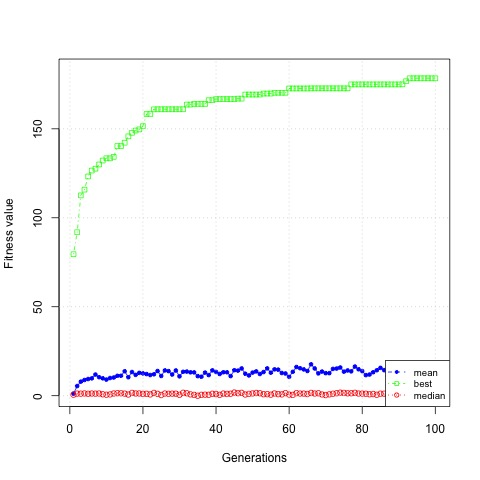
\includegraphics[width=3in]{{{inc/results/custom-crossover}}}\quad
    }
    }
    \caption{Porównanie domyślnej funkcji krzyżowania z własną}
    \end{figure}
     \begin{figure}[!h]
    \centering
    \mbox{
    \subfigure{
    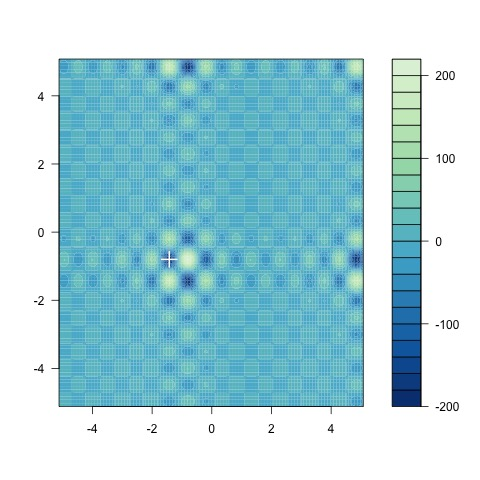
\includegraphics[width=3in]{{{inc/results/default_ga_result}}}\quad
    }
    \subfigure{
    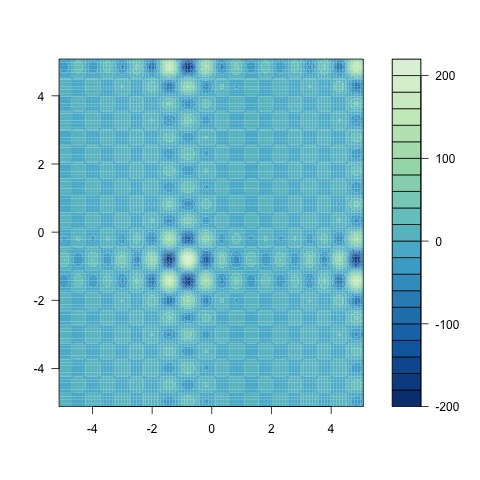
\includegraphics[width=3in]{{{inc/results/custom-crossover-result}}}\quad
    }
    }
    \caption{Porównanie domyślnej funkcji krzyżowania z własną  - znalezione ekstrema}
    \end{figure}

W przypadku własnej funkcji krzyżującej algorytm nie znalazł ekstremum globalnego. Wartości średniej i mediany spadły znaczącą w stosunku do domyślnej implementacji. Mediana jest praktycznie równa zero. Algorytm prawdopodobnie znalazł minimum lokalne i nie mógł odnaleźć lepszych rozwiązań, mimo wybierania lepszej wartości \textit{fitness}, ponieważ do każdego rodzica jest dodawana wartość losowa z przedziału [-1, 1]. Prawdopodobnie gdyby ten przedział był większy algorytm mógłby wylosować lepszego rodzica, który nie znajduje się w lokalnym minimum.

\clearpage
\section{Problem komiwojażera}

\subsection{Opis problemu}
Problem komiwojażera jest jednym z najsłynniejszych problemów informatyki i badań operacyjnych. Często nazywa się skrótem TSP, skrót nazwy angielskiej nazwy "podróżujący sprzedawca". Można go sformułować w następujący sposób:
"Biorąc pod uwagę n miast wraz z odległością między każdą parą tych miast, znajdź najkrótszą trasę, która przebiega przez każde miasto dokładnie raz."

\clearpage
\subsection{Instancja 1 - \textit{bays29}}

\subsubsection{Zmiana parametru krzyżowania}
Zwiększanie parametru krzyżowania zmniejsza wartość średniej i mediany, oznacza to, że średnie wyniki w populacji są coraz gorsze. Algorytm znalazł najlepsze rozwiązanie dla wartości parametru 0.5. 

  \begin{figure}[!htbp]
    \centering
    \mbox{
    \subfigure{
     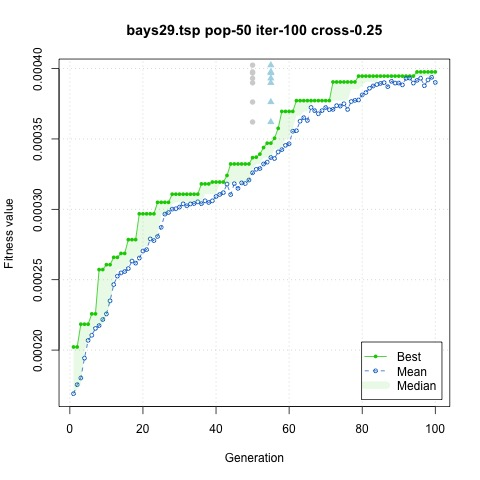
\includegraphics[width=3in]{{{inc/results/learning-curve/bays29.tsp-pop-50-iter-100-cross-0.25}}}\quad
    }
    \subfigure{
   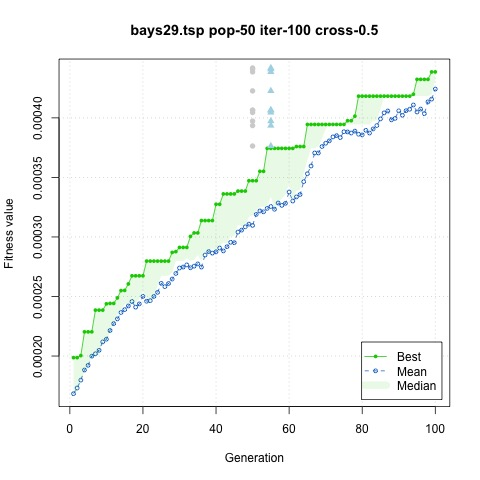
\includegraphics[width=3in]{{{inc/results/learning-curve/bays29.tsp-pop-50-iter-100-cross-0.5}}}\quad
  }
    }
        \mbox{
    \subfigure{
     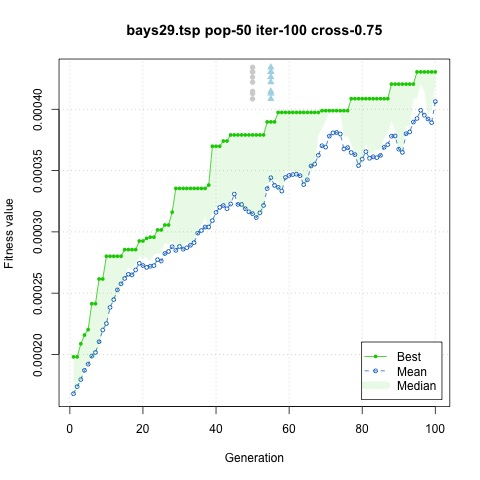
\includegraphics[width=3in]{{{inc/results/learning-curve/bays29.tsp-pop-50-iter-100-cross-0.75}}}\quad
    }
    \subfigure{
   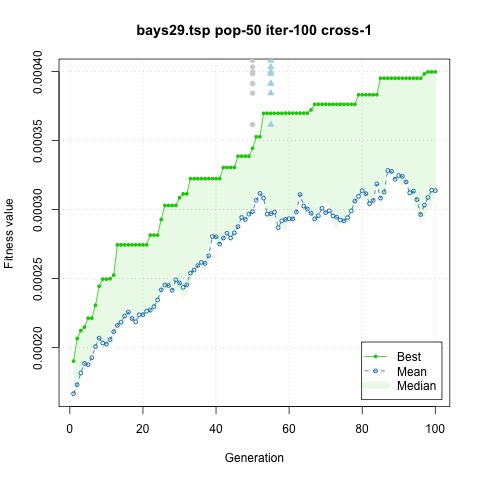
\includegraphics[width=3in]{{{inc/results/learning-curve/bays29.tsp-pop-50-iter-100-cross-1}}}\quad
  }
    }
    \caption{Porównanie wyników podczas zmiany parametru krzyżowania}
    \end{figure}
    
    \clearpage
\subsubsection{Zmiana parametru liczby pokoleń}

Zwiększanie parametru liczby pokoleń zwiększa wartość znajdowanego rozwiązania. Poziom wartości średniej i mediany są bliskie najlepszemu rozwiązaniu.

\begin{figure}[!htbp]
    \centering
    \mbox{
    \subfigure{
     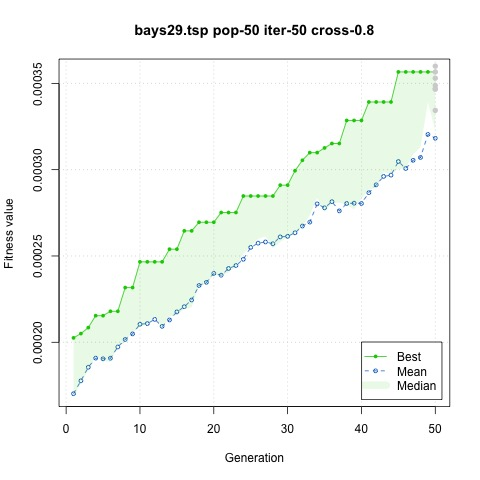
\includegraphics[width=3in]{{{inc/results/learning-curve/bays29.tsp_pop-50_iter-50_cross-0.8}}}\quad
    }
    \subfigure{
   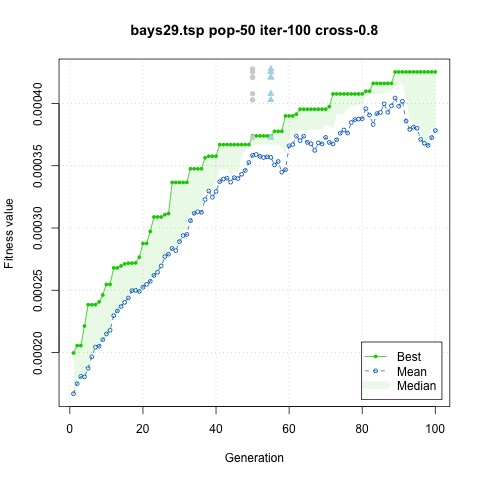
\includegraphics[width=3in]{{{inc/results/learning-curve/bays29.tsp-pop-50-iter-100-cross-0.8}}}\quad
  }
    }
        \mbox{
    \subfigure{
     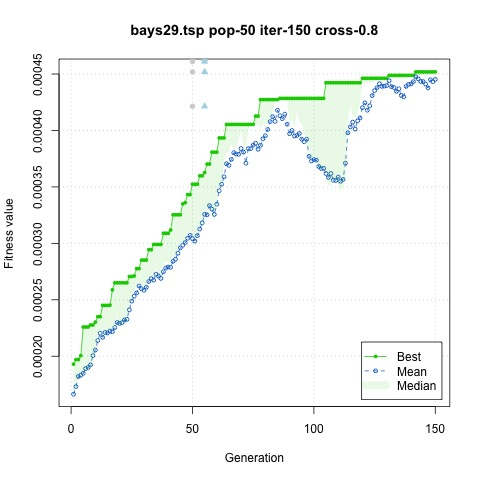
\includegraphics[width=3in]{{{inc/results/learning-curve/bays29.tsp-pop-50-iter-150-cross-0.8}}}\quad
    }
    \subfigure{
   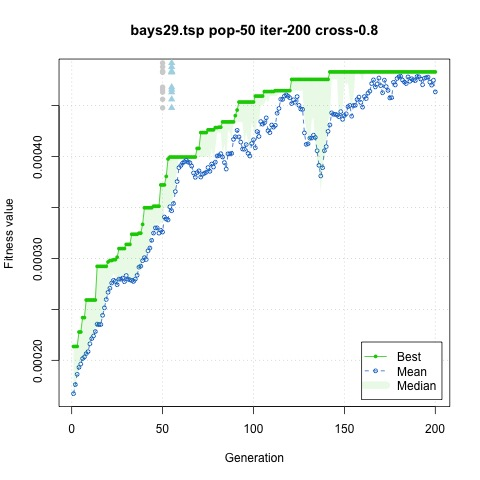
\includegraphics[width=3in]{{{inc/results/learning-curve/bays29.tsp-pop-50-iter-200-cross-0.8}}}\quad
  }
    }
    \caption{Porównanie wyników podczas zmiany parametru liczby pokoleń}
    \end{figure}
    
 \clearpage
\subsubsection{Zmiana parametru rozmiaru populacji}

Wraz ze wzrostem ilości osobników w pokoleniu algorytm znajduje coraz lepsze rozwiązania. Wartość średniej i mediany maleje wraz ze wzrostem rozmiaru populacji. 
\begin{figure}[!h]
    \centering
    \mbox{
    \subfigure{
     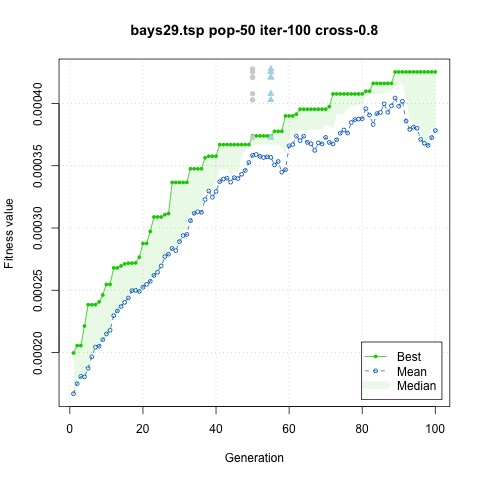
\includegraphics[width=3in]{{{inc/results/learning-curve/bays29.tsp-pop-50-iter-100-cross-0.8}}}\quad
    }
    \subfigure{
   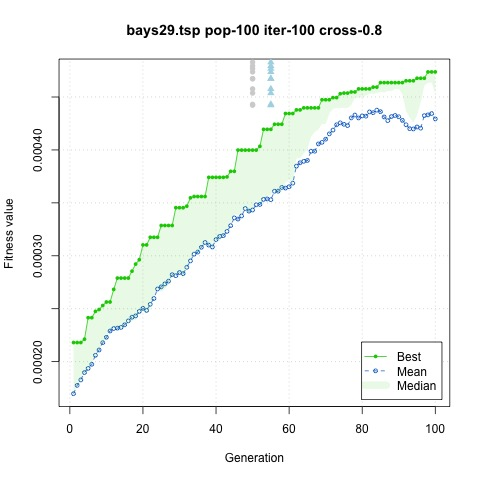
\includegraphics[width=3in]{{{inc/results/learning-curve/bays29.tsp-pop-100-iter-100-cross-0.8}}}\quad
  }
    }
        \mbox{
    \subfigure{
     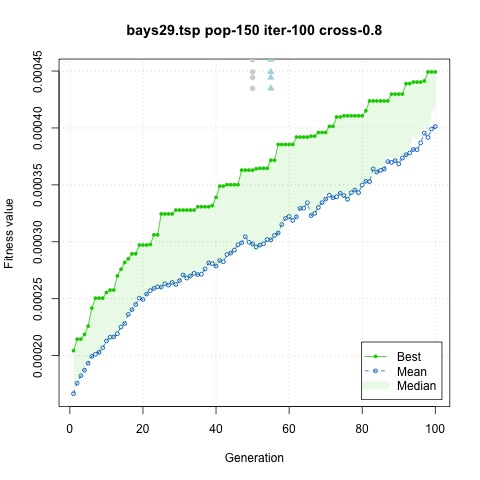
\includegraphics[width=3in]{{{inc/results/learning-curve/bays29.tsp-pop-150-iter-100-cross-0.8}}}\quad
    }
    \subfigure{
   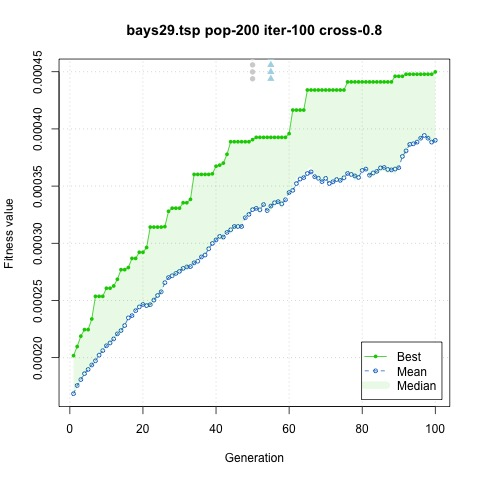
\includegraphics[width=3in]{{{inc/results/learning-curve/bays29.tsp-pop-200-iter-100-cross-0.8}}}\quad
  }
    }
    \caption{Porównanie wyników podczas zmiany parametru rozmiaru populacji}
    \end{figure}
  
  \clearpage
\subsubsection{Jednoczesna zmiana krzyżowania i mutacji oraz rozmiaru populacji i liczby pokoleń}

Algorytm uzyskał najlepszy wynik gdy populacja wynosiła 100, a liczba pokoleń 80. Analiza wykresu temperaturowego jednoczesnej zmiany mutowania i krzyżowania nie pozwala wysunąć jednoznacznych wniosków. Można wydzielić dwa obszary parametrów dla których algorytm znalazł lepsze rozwiązanie: krzyżowanie 0.6 i mutacja 0.4 oraz krzyżowanie 0.8 i mutacja 0.75

\begin{figure}[!h]
    \centering
        \mbox{
    \subfigure{
     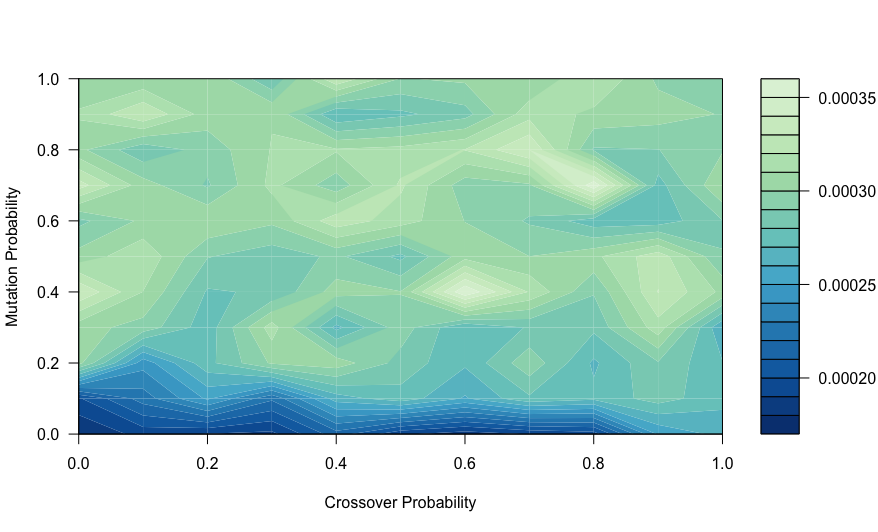
\includegraphics[width=3in]{{{inc/results/tsp/bays29_mutation_crossover_temperature}}}\quad
    }
    \subfigure{
   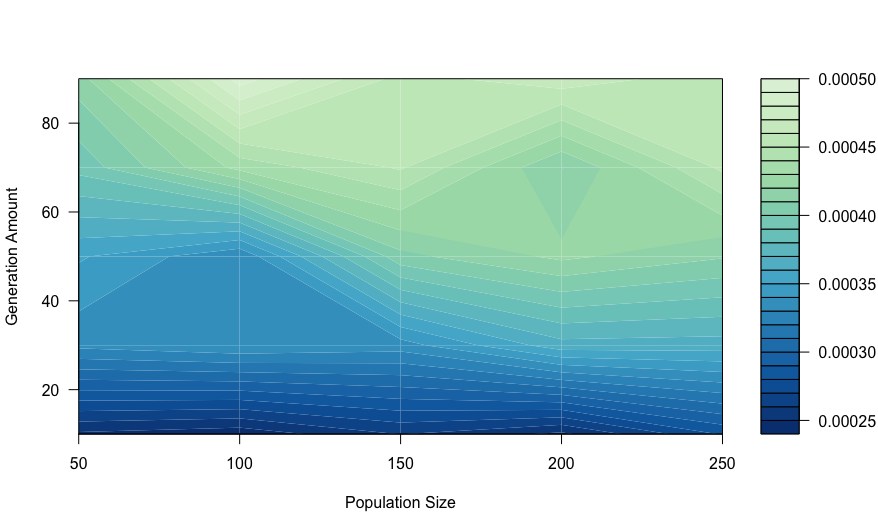
\includegraphics[width=3in]{{{inc/results/tsp/bays29_population_iteration_temperature}}}\quad
  }
    }
    \caption{Porównanie wyników podczas jednoczesnej zmiany parametrów}
    \end{figure}

%%%%%%%%%%%%%%%%%%%%%%%%%%%%%%%%%%%%%%%%%%%%%%%%%%%%%%%
\clearpage
\subsection{Instancja 2 - \textit{gr17}}
Średnie wartości są zbliżone do najlepszego rozwiązania dla najmniejszych wartości parametru krzyżowania. Wzrost tego parametru skutkuje zmniejszeniem średniej wyników w każdej populacji.
\subsubsection{Zmiana parametru krzyżowania}
  \begin{figure}[!h]
    \centering
    \mbox{
    \subfigure{
     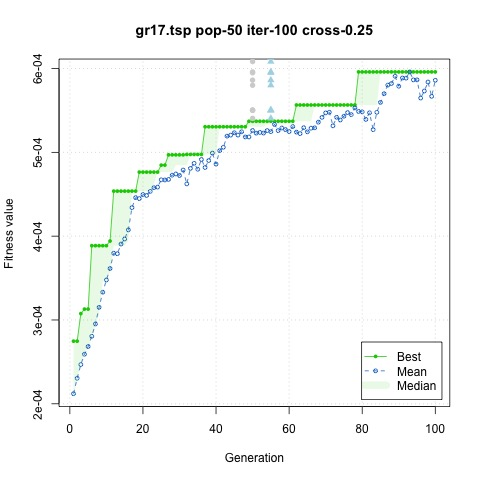
\includegraphics[width=3in]{{{inc/results/learning-curve/gr17.tsp-pop-50-iter-100-cross-0.25}}}\quad
    }
    \subfigure{
   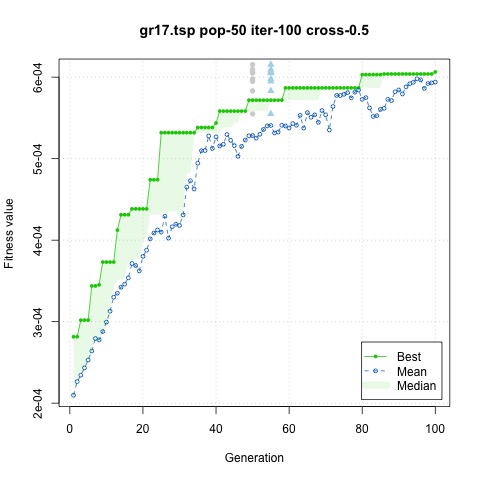
\includegraphics[width=3in]{{{inc/results/learning-curve/gr17.tsp-pop-50-iter-100-cross-0.5}}}\quad
  }
    }
        \mbox{
    \subfigure{
     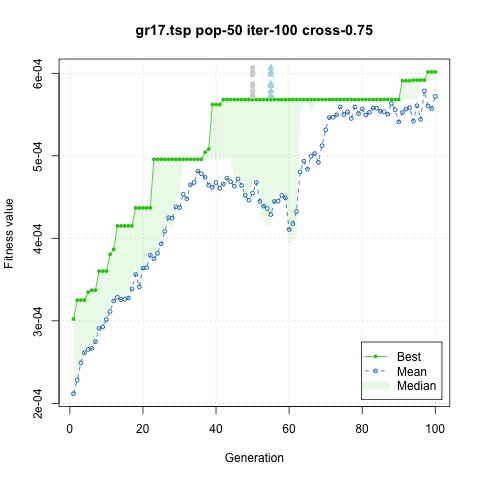
\includegraphics[width=3in]{{{inc/results/learning-curve/gr17.tsp-pop-50-iter-100-cross-0.75}}}\quad
    }
    \subfigure{
   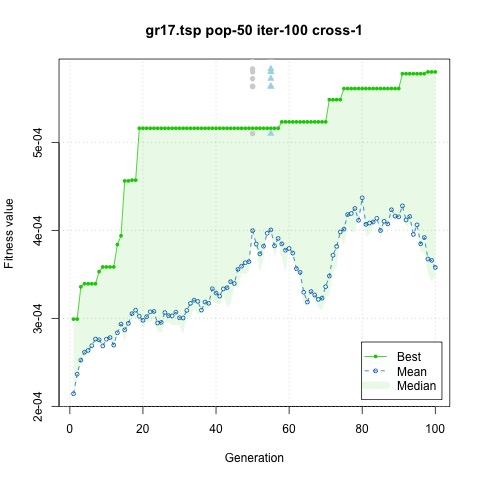
\includegraphics[width=3in]{{{inc/results/learning-curve/gr17.tsp-pop-50-iter-100-cross-1}}}\quad
  }
    }
    \caption{Porównanie wyników podczas zmiany parametru krzyżowania}
    \end{figure}
    
    
     \clearpage
\subsubsection{Zmiana parametru liczby pokoleń}

Wzrost parametru liczby pokoleń jest jednoznaczny ze wzrostem wartości najlepszego rozwiązania. Zmniejsza się również wartość średnia i mediana. 

\begin{figure}[!h]
    \centering
    \mbox{
    \subfigure{
     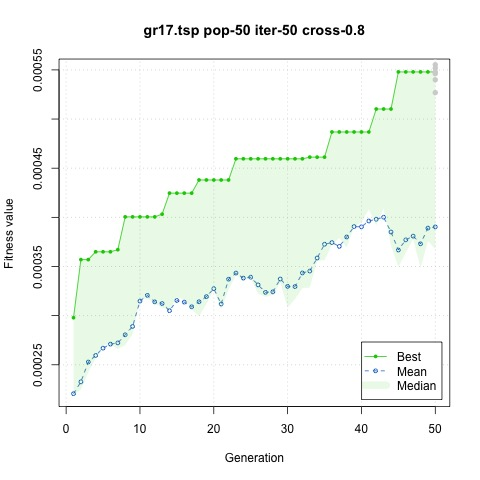
\includegraphics[width=3in]{{{inc/results/learning-curve/gr17.tsp-pop-50-iter-50-cross-0.8}}}\quad
    }
    \subfigure{
   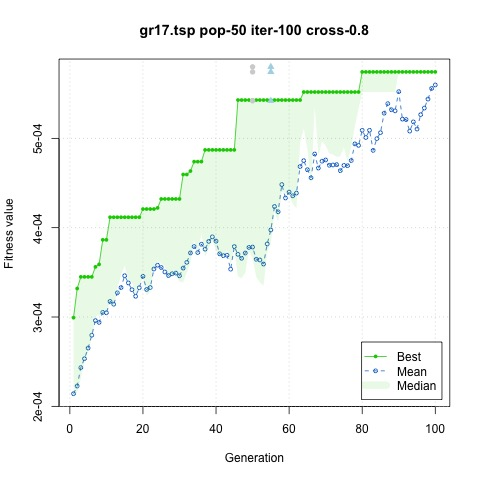
\includegraphics[width=3in]{{{inc/results/learning-curve/gr17.tsp-pop-50-iter-100-cross-0.8}}}\quad
  }
    }
        \mbox{
    \subfigure{
     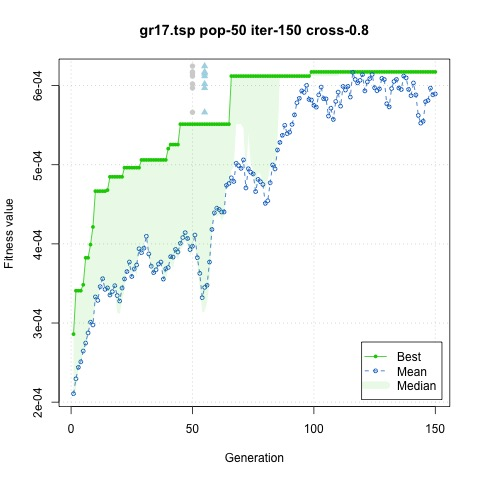
\includegraphics[width=3in]{{{inc/results/learning-curve/gr17.tsp-pop-50-iter-150-cross-0.8}}}\quad
    }
    \subfigure{
   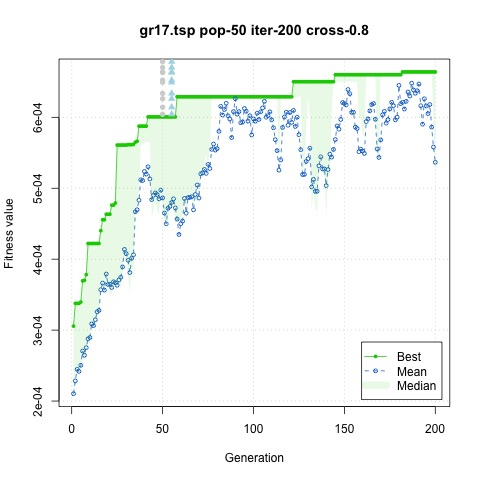
\includegraphics[width=3in]{{{inc/results/learning-curve/gr17.tsp-pop-50-iter-200-cross-0.8}}}\quad
  }
    }
    \caption{Porównanie wyników podczas zmiany parametru liczby pokoleń}
    \end{figure}
    
    
    \clearpage
\subsubsection{Zmiana parametru rozmiaru populacji}

Wartość znajdowanego rozwiązania jest na stałym poziomie niezależnie od ilości osobników. Zmniejsza się jednak średnia wartość dla każdego pokolenia. 
\begin{figure}[!h]
    \centering
    \mbox{
    \subfigure{
     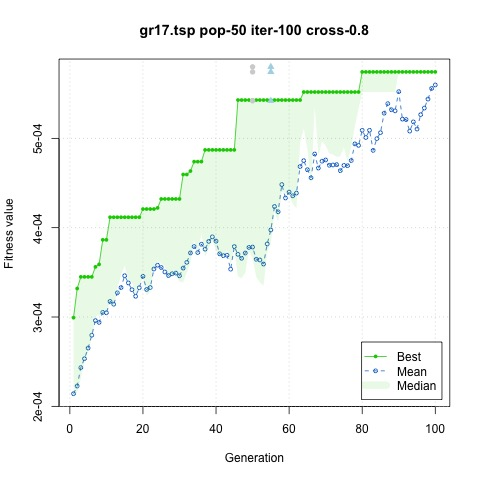
\includegraphics[width=3in]{{{inc/results/learning-curve/gr17.tsp-pop-50-iter-100-cross-0.8}}}\quad
    }
    \subfigure{
   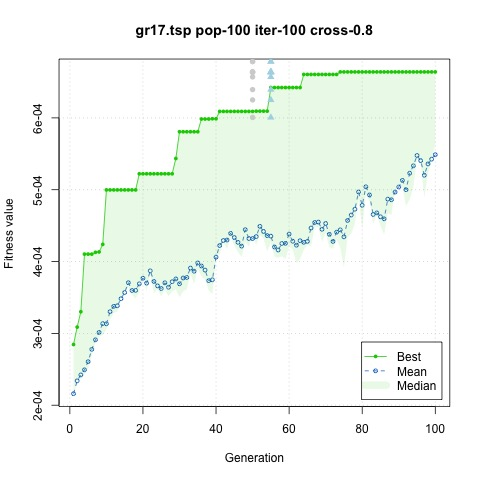
\includegraphics[width=3in]{{{inc/results/learning-curve/gr17.tsp-pop-100-iter-100-cross-0.8}}}\quad
  }
    }
        \mbox{
    \subfigure{
     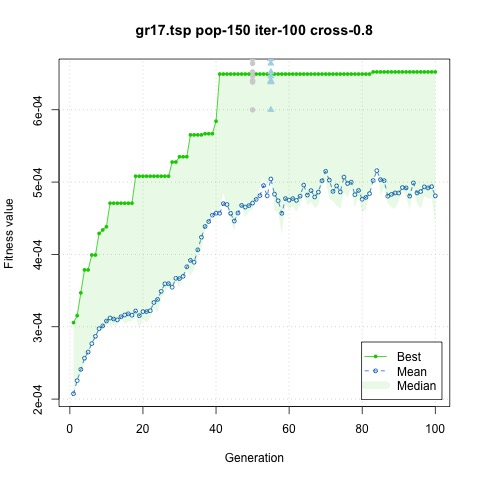
\includegraphics[width=3in]{{{inc/results/learning-curve/gr17.tsp-pop-150-iter-100-cross-0.8}}}\quad
    }
    \subfigure{
   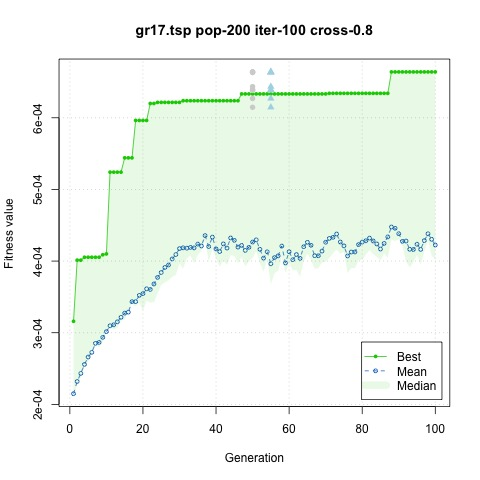
\includegraphics[width=3in]{{{inc/results/learning-curve/gr17.tsp-pop-200-iter-100-cross-0.8}}}\quad
  }
    }
    \caption{Porównanie wyników podczas zmiany parametru rozmiaru populacji}
    \end{figure}
    
    
    \clearpage
\subsubsection{Jednoczesna zmiana krzyżowania i mutacji oraz rozmiaru populacji i liczby pokoleń}

Dla tej instancji nie znaleziono korelacji między jednoczesną zmianą wartości krzyżowania i mutacji a polepszeniem uzyskiwanego wyniku. Najlepszy wynik uzyskano dla wartości krzyżowania 0.8 i mutacji 0.1.

\begin{figure}[!h]
    \centering
    \subfigure{
     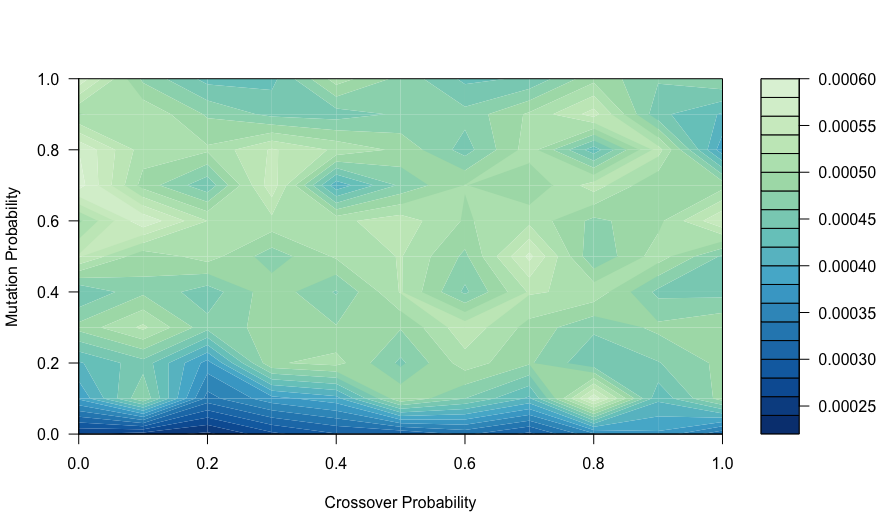
\includegraphics[width=3in]{{{inc/results/tsp/gr17_mutation_crossover_temperature}}}\quad
    }
    \caption{Porównanie wyników podczas jednoczesnej zmiany parametrów}
    \end{figure}

Dla jednoczesnej zmiany rozmiaru populacji i liczby iteracji najlepszy wynik uzyskano dla 100 osobników i 75 pokoleń.

\begin{figure}[!h]
    \centering
    \subfigure{
   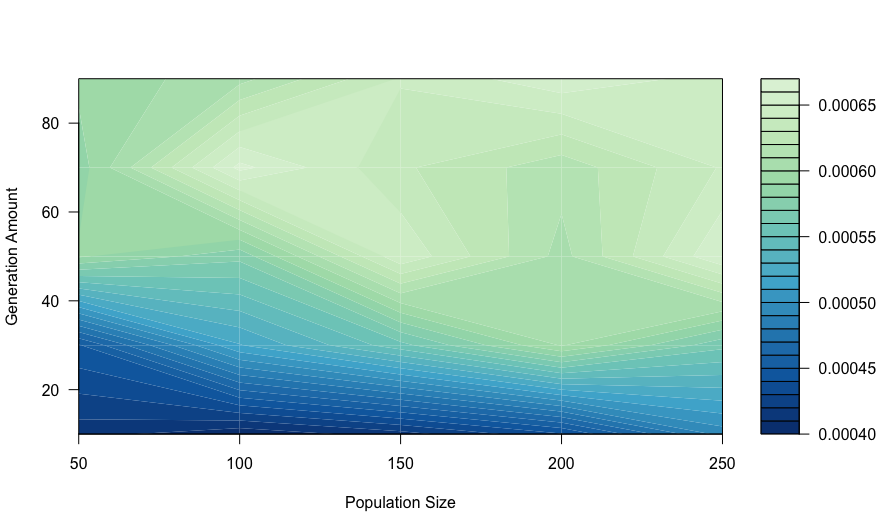
\includegraphics[width=3in]{{{inc/results/tsp/gr17_population_iteration_temperature}}}\quad
  }
    \caption{Porównanie wyników podczas jednoczesnej zmiany parametrów}
    \end{figure}


%%%%%%%%%%%%%%%%%%%%%%%%%%%%%%%%%%%%%%%%%%%%%%%%%
\clearpage
\subsection{Instancja 3 - \textit{gr120}}

Średnie wartości są zbliżone do najlepszego rozwiązania dla najmniejszych wartości parametru krzyżowania. Wzrost tego parametru skutkuje zmniejszeniem średniej wyników w każdej populacji.

\subsubsection{Zmiana parametru krzyżowania}
  \begin{figure}[!h]
    \centering
    \mbox{
    \subfigure{
     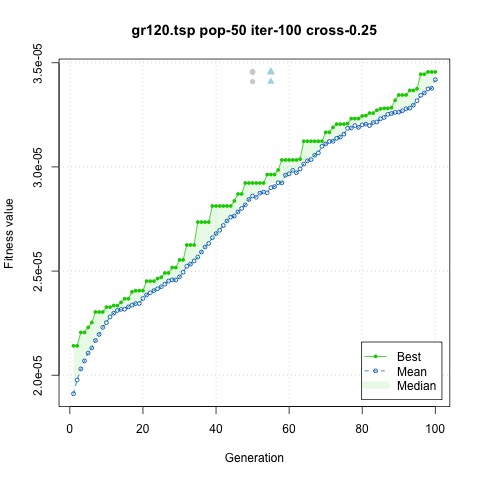
\includegraphics[width=3in]{{{inc/results/learning-curve/gr120.tsp-pop-50-iter-100-cross-0.25}}}\quad
    }
    \subfigure{
   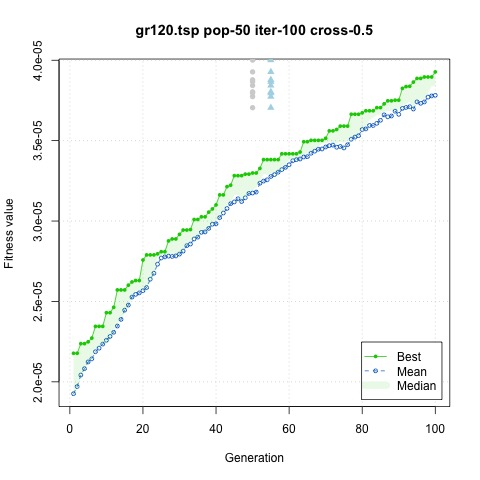
\includegraphics[width=3in]{{{inc/results/learning-curve/gr120.tsp-pop-50-iter-100-cross-0.5}}}\quad
  }
    }
        \mbox{
    \subfigure{
     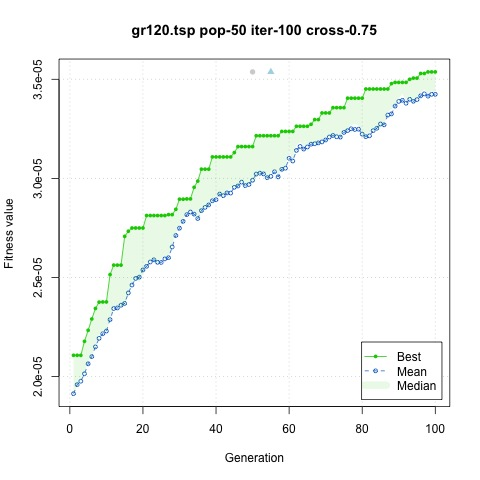
\includegraphics[width=3in]{{{inc/results/learning-curve/gr120.tsp-pop-50-iter-100-cross-0.75}}}\quad
    }
    \subfigure{
   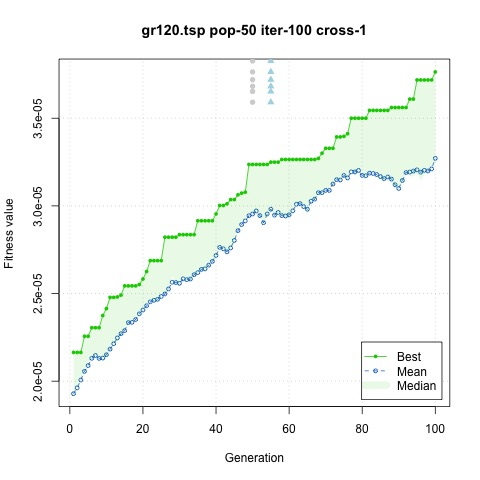
\includegraphics[width=3in]{{{inc/results/learning-curve/gr120.tsp-pop-50-iter-100-cross-1}}}\quad
  }
    }
    \caption{Porównanie wyników podczas zmiany parametru krzyżowania}
    \end{figure}
     
     
     \clearpage
\subsubsection{Zmiana parametru liczby pokoleń}

Wzrost parametru liczby pokoleń jest jednoznaczny ze wzrostem wartości najlepszego rozwiązania. Zmniejsza się również wartość średnia i mediana. 


\begin{figure}[!h]
    \centering
    \mbox{
    \subfigure{
     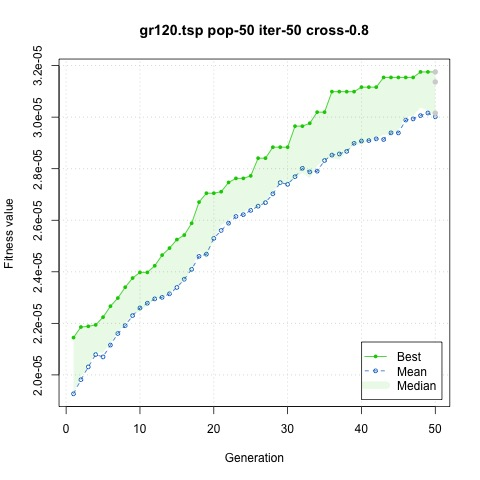
\includegraphics[width=3in]{{{inc/results/learning-curve/gr120.tsp-pop-50-iter-50-cross-0.8}}}\quad
    }
    \subfigure{
   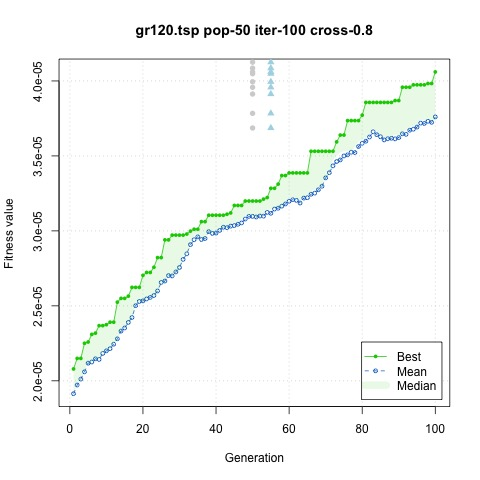
\includegraphics[width=3in]{{{inc/results/learning-curve/gr120.tsp-pop-50-iter-100-cross-0.8}}}\quad
  }
    }
        \mbox{
    \subfigure{
     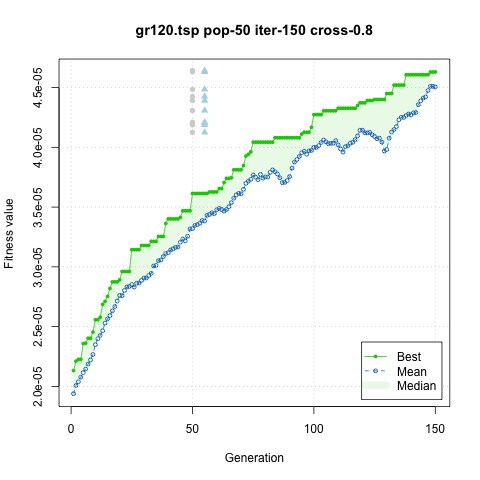
\includegraphics[width=3in]{{{inc/results/learning-curve/gr120.tsp-pop-50-iter-150-cross-0.8}}}\quad
    }
    \subfigure{
   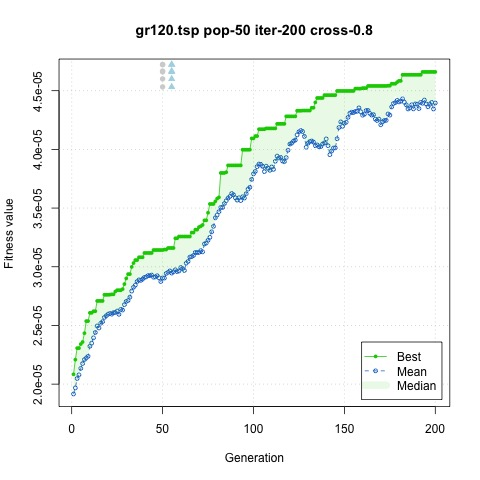
\includegraphics[width=3in]{{{inc/results/learning-curve/gr120.tsp-pop-50-iter-200-cross-0.8}}}\quad
  }
    }
    \caption{Porównanie wyników podczas zmiany parametru liczby pokoleń}
    \end{figure}
    
    \clearpage
\subsubsection{Zmiana parametru rozmiaru populacji}

Wartość znajdowanego rozwiązania jest na stałym poziomie niezależnie od ilości osobników. Zmniejsza się jednak średnia wartość dla każdego pokolenia. 

\begin{figure}[!h]
    \centering
    \mbox{
    \subfigure{
     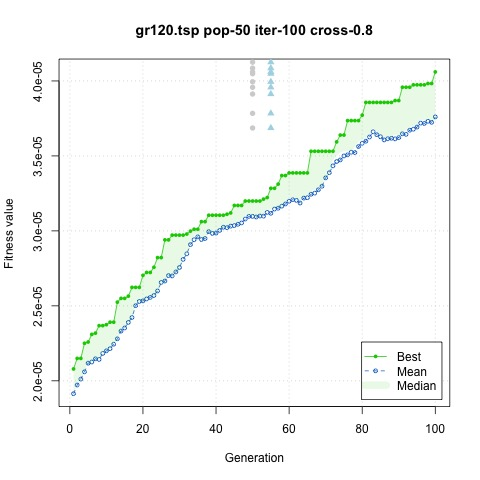
\includegraphics[width=3in]{{{inc/results/learning-curve/gr120.tsp-pop-50-iter-100-cross-0.8}}}\quad
    }
    \subfigure{
   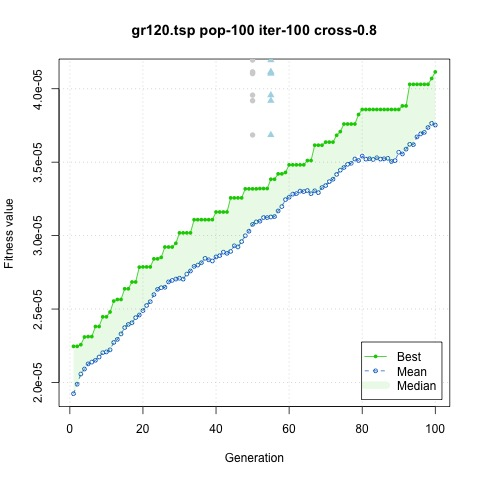
\includegraphics[width=3in]{{{inc/results/learning-curve/gr120.tsp-pop-100-iter-100-cross-0.8}}}\quad
  }
    }
        \mbox{
    \subfigure{
     \includegraphics[width=3in]{{{inc/results/learning-curve/gr120.tsp-pop-150-iter-100-cross-0.8}}}\quad
    }
    \subfigure{
   \includegraphics[width=3in]{{{inc/results/learning-curve/gr120.tsp-pop-200-iter-100-cross-0.8}}}\quad
  }
    }
    \caption{Porównanie wyników podczas zmiany parametru rozmiaru populacji}
    \end{figure}
    
    \clearpage
\subsubsection{Jednoczesna zmiana krzyżowania i mutacji oraz rozmiaru populacji i liczby pokoleń}


Dla tej instancji nie znaleziono korelacji między jednoczesną zmianą wartości krzyżowania i mutacji a polepszeniem uzyskiwanego wyniku. 


\begin{figure}[!h]
    \centering
    \subfigure{
     \includegraphics[width=3in]{{{inc/results/tsp/gr120_mutation_crossover_temperature}}}\quad
    }
    \caption{Porównanie wyników podczas jednoczesnej zmiany parametrów}
    \end{figure}

Dla jednoczesnej zmiany rozmiaru populacji i liczby iteracji najlepszy wynik uzyskano dla 150 osobników i 50 pokoleń.

\begin{figure}[!h]
    \centering
    \subfigure{
   \includegraphics[width=3in]{{{inc/results/tsp/gr120_population_iteration_temperature}}}\quad
  }
    \caption{Porównanie wyników podczas jednoczesnej zmiany parametrów}
    \end{figure}
    
    \clearpage
    \section{HGA}
    
    
    \clearpage
\section{Wnioski}

Implementacja własnych funkcji mutowania i krzyżowania jest  zadaniem nietrywialnym, ale możliwym do wykonania.  Jakość wyników uzyskanych przy własnych implementacjach znacząco odbiega od domyślnych funkcji.


\section{Literatura}
\begin{enumerate}
\item Artur Suchwałko, "Wprowadzenie do R dla programistow innych jezykow", \url{https://cran.r-project.org/doc/contrib/R-dla-programistow-innych-jezykow.pdf}, 2014-02-23
\item Luca Scrucca, "On some extensions to GA package:
hybrid optimisation, parallelisation and islands evolution", \url{https://arxiv.org/pdf/1605.01931.pdf}, 2016-05-09
\item dr inż. Julian Sienkiewicz, "Pakiet R w analizie układów złożonych", \url{http://www.if.pw.edu.pl/~julas/CSAR/csar11.html}, 2017
\item W. N. Venables, D. M. Smith, R Core Team, "An Introduction to R", \url{https://cran.r-project.org/doc/manuals/r-release/R-intro.pdf}, 2018-04-23
\item Luca Scrucca, "Package 'GA'", \url{ftp://cran.r-project.org/pub/R/web/packages/GA/GA.pdf}, 2016-09-29
\item Katharine Mullen, "Package 'globalOptTests'", \url{https://cran.r-project.org/web/packages/globalOptTests/globalOptTests.pdf},
2015-02-15
\item Abdal-Rahman Hedar, "Global Optimization Test Problems", \url{http://www-optima.amp.i.kyoto-u.ac.jp/member/student/hedar/Hedar_files/TestGO.htm}, dostęp online: 2018-05-04
\end{enumerate}



\end{document}\documentclass{article}
